% TEMPLATE : FICHE DE REVISION
\documentclass[11pt]{article}

\usepackage[french]{babel}
\usepackage[T1]{fontenc}
\usepackage{graphicx}
\usepackage{framed}
\usepackage{float}
\usepackage[normalem]{ulem}
\usepackage{indentfirst}
\usepackage{amsmath,amsthm,amssymb,amsfonts}
\usepackage[italicdiff]{physics}
\usepackage{wrapfig}
\usepackage{lmodern,mathrsfs}
\usepackage{caption}
\usepackage{subcaption}
\usepackage[dvipsnames]{xcolor}
\usepackage[utf8]{inputenc}
\usepackage[a4paper, top=0.5in,bottom=0.5in, left=0.7in, right=0.7in, footskip=0.3in, includefoot]{geometry}
\usepackage[most]{tcolorbox}
\usepackage{multicol}
\usepackage{tabularx}
\usepackage{setspace}
\usepackage{gensymb}
\usepackage{titlesec}
\usepackage[unicode,psdextra]{hyperref}
\pdfstringdefDisableCommands{\def\varepsilon{\textepsilon}}
\usepackage{pgfplots}
\usepackage{bookmark}
\hypersetup{
	colorlinks,
	citecolor=black,
	filecolor=black,
	linkcolor=black,
	urlcolor=black
}

\graphicspath{ {./image} } 

\titleformat*{\section}{\large\bfseries}

\renewcommand{\phi}{\varphi}
\newcommand{\C}{\mathbb{C}}
\newcommand{\K}{\mathbb{K}}
\newcommand{\N}{\mathbb{N}}
\newcommand{\Q}{\mathbb{Q}}
\newcommand{\R}{\mathbb{R}}
\newcommand{\Ne}{\mathbb{N}^{*}}
\newcommand{\Os}[1][]{\underset{#1}{\mathcal{O}}}
\newcommand{\integral}[2]{\ensuremath{\int_{#1}^{#2}}}
\newcommand{\deriv}[3][]{\ensuremath{\frac{d^{#1}#2}{d#3}}}
\let\spn\relax\let\Re\relax\let\Im\relax
\DeclareMathOperator{\Re}{\text{Re}}
\DeclareMathOperator{\Im}{\text{Im}}

\newtheoremstyle{mystyle}{}{}{}{}{\sffamily\bfseries}{.}{ }{}
\newtheoremstyle{cstyle}{}{}{}{}{\sffamily\bfseries}{.}{ }{\thmnote{#3}}
\makeatletter
\renewcommand\qedsymbol{}
\makeatother

\theoremstyle{cstyle}{\newtheorem{definition}{Définition}[section]}
\theoremstyle{cstyle}{\newtheorem{proposition}[definition]{Propriété}}
\theoremstyle{cstyle}{\newtheorem{theorem}[definition]{Théorème}}
\theoremstyle{mystyle}{\newtheorem{lemma}[definition]{Lemme}}
\theoremstyle{mystyle}{\newtheorem{corollary}[definition]{Corollaire}}
\theoremstyle{mystyle}{\newtheorem*{remark}{Remarque}}
\theoremstyle{mystyle}{\newtheorem*{remarks}{Remarques}}
\theoremstyle{mystyle}{\newtheorem*{example}{Exemple}}
\theoremstyle{mystyle}{\newtheorem*{examples}{Exemples}}
\theoremstyle{definition}{\newtheorem*{exercise}{Exercice}}
\theoremstyle{mystyle}{\newtheorem*{methode}{Méthode}}
\theoremstyle{cstyle}{\newtheorem*{cthm}{}}

%Warning environment
\newtheoremstyle{warn}{}{}{}{}{\normalfont}{}{ }{}
\theoremstyle{warn}
\newtheorem*{warning}{\warningsign{0.2}\relax}

%Symbol for the warning environment, designed to be easily scalable
\newcommand{\warningsign}[1]{\tikz[scale=#1,every node/.style={transform shape}]{\draw[-,line width={#1*0.8mm},red,fill=yellow,rounded corners={#1*2.5mm}] (0,0)--(1,{-sqrt(3)})--(-1,{-sqrt(3)})--cycle;
		\node at (0,-1) {\fontsize{48}{60}\selectfont\bfseries!};}}

\tcolorboxenvironment{definition}{boxrule=0pt,boxsep=0pt,colback={white},colframe=white,left=8pt,right=8pt,enhanced jigsaw, borderline west={2pt}{0pt}{red},sharp corners,before skip=10pt,after skip=10pt,breakable}
\tcolorboxenvironment{proposition}{boxrule=0pt,boxsep=0pt,colback={white},left=8pt,colframe=white,right=8pt,enhanced jigsaw, borderline west={2pt}{0pt}{Cyan},sharp corners,before skip=10pt,after skip=10pt,breakable}
\tcolorboxenvironment{theorem}{boxrule=0pt,boxsep=0pt,colback={white}, colframe = white, left=8pt,right=8pt,enhanced jigsaw, borderline west={2pt}{0pt}{blue},sharp corners,before skip=10pt,after skip=10pt,breakable}
\tcolorboxenvironment{lemma}{boxrule=0pt,boxsep=0pt,colback={Cyan!10},left=8pt,right=8pt,enhanced jigsaw, borderline west={2pt}{0pt}{Cyan},sharp corners,before skip=10pt,after skip=10pt,breakable}
\tcolorboxenvironment{corollary}{boxrule=0pt,boxsep=0pt,colback={violet!10},left=8pt,right=8pt,enhanced jigsaw, borderline west={2pt}{0pt}{violet},sharp corners,before skip=10pt,after skip=10pt,breakable}
\tcolorboxenvironment{proof}{boxrule=0pt,boxsep=0pt,colback={white},colframe=white,borderline west={2pt}{0pt}{Green!80},enhanced jigsaw,left=8pt,right=8pt,sharp corners,before skip=10pt,after skip=10pt,breakable}
\tcolorboxenvironment{remark}{boxrule=0pt,boxsep=0pt,blanker,borderline west={2pt}{0pt}{CadetBlue!80},left=8pt,right=8pt,before skip=10pt,after skip=10pt,breakable}
\tcolorboxenvironment{remarks}{boxrule=0pt,boxsep=0pt,blanker,borderline west={2pt}{0pt}{Green},left=8pt,right=8pt,before skip=10pt,after skip=10pt,breakable}
\tcolorboxenvironment{example}{boxrule=0pt,boxsep=0pt,blanker,borderline west={2pt}{0pt}{Black},left=8pt,right=8pt,sharp corners,before skip=10pt,after skip=10pt,breakable}
\tcolorboxenvironment{examples}{boxrule=0pt,boxsep=0pt,blanker,borderline west={2pt}{0pt}{Black},left=8pt,right=8pt,sharp corners,before skip=10pt,after skip=10pt,breakable}
\tcolorboxenvironment{cthm}{boxrule=0pt,boxsep=0pt,colback={gray!10},left=8pt,right=8pt,enhanced jigsaw, borderline west={2pt}{0pt}{gray},sharp corners,before skip=10pt,after skip=10pt,breakable}
\tcolorboxenvironment{methode}{boxrule=0pt,boxsep=0pt,colback={Aquamarine!10},left=8pt,right=8pt,enhanced jigsaw, borderline west={2pt}{0pt}{Aquamarine},sharp corners,before skip=10pt,after skip=10pt,breakable}

\setlength{\parindent}{0.2in}
\setlength{\parskip}{0pt}
\setlength{\columnseprule}{0pt}

%\renewcommand{\arraystretch}{1.5}


\title{Chapitre 14 : Transferts d'énergie}
\author{}
\date{}

\setstretch{1.4}

\begin{document}
	
	\maketitle
	
	\begin{minipage}[t]{0.45\textwidth}
		\section{Premier principe de la thermodynamique}
		
		\subsection{Transferts thermiques}
		\begin{definition}[Système isolé]
			Un système est isolé s'il n'a aucune interaction avec l'exterieur.
		\end{definition}
		\begin{definition}[Transfert thermique, ou chaleur]
			Deux systèmes côte à côte peuvent échanger un \textbf{transfert thermique} à travers une \underline{paroi immobile}. Ils sont alors en \textbf{contact thermique}.
		\end{definition}
	
		\begin{definition}[Paroi diatherme / calorifugée]
			Une paroi est \textbf{diatherme} si elle permet le transfert thermique.
			
			Une paroi est \textbf{calorifugée} si elle ne permet aucun transfert thermique.
		\end{definition}
	
		\begin{definition}[Évolution adiabatique]
			Un système qui n'a aucun échange thermique avec l'extérieur a une évolution adiabatique.
		\end{definition}
	
		\begin{proposition}[Équilibre thermique]
			Lorsque deux systèmes sont en \underline{contact thermique}, l'équilibre thermique est atteint lorsque les deux ont la même température.
		\end{proposition}
	
	\end{minipage}
	\hfill
	\vrule
	\hfill
	\begin{minipage}[t]{0.45\textwidth}
		\subsection{Travail}
		
		\begin{definition}[Travail]
			Un \textbf{travail} est un \underline{échange d'énergie} dû à une action extérieure sur des grandeurs variables du système.
		\end{definition}
	
		\begin{proposition}[Travail d'une force]
			Une force extérieur \(\vec{F}\) d'appliquant en un point \(M\) du système fournit au système un travail infinitésimal \fbox{\(\delta W = \vec{F} \cdot \text{d}\vec{OM}\)} ou encore un travail \fbox{\(W = \int \vec{F}.\text{d}\vec{OM}\)}
		\end{proposition}
	
		\begin{proposition}[Travail des forces de pression]
			Un système soumis à une pression \(P_{ext}\) et dont le volume varie de d\(V\) reçoit un travail \(\delta W = -P_{ext}.\text{d}V\). Le travail total reçu des forces exterieures vaut donc :
			\[
				W = - \int P_{ext}.\text{d}V 
			\] 
		\end{proposition}
	
		\begin{proposition}[Équilibre mécanique de pression]
			Si deux systèmes sont séparés par une \underline{paroi mobile libre} (déplacement sans frottements) et de masse négligeable, l'équilibre mécanique est atteint lorsque les \textbf{pressions} des deux systèmes est égale.
		\end{proposition}
	
		\begin{proof}
			On utilise le cas d'un piston en $1D$ à l'horizontale.
		\end{proof}
	
	\end{minipage}

	\newpage
	\begin{minipage}[t]{0.45\textwidth}
		\begin{proposition}[Travail électrique]
			Si un système reçoit un courant $i$ de la part d'un générateur de tension extérieur de tension $e$, alors on a \fbox{\(\delta W = e \cdot i \cdot \text{d}t = e \cdot \text{d}q\)}
		\end{proposition}
	
		\subsection{Premier principe}
		
		\begin{definition}[Énergie interne]
			Pour tout système thermodynamique à l'équilibre, on peut définir une fonction d'état \(U\) appelé \textbf{énergie interne} qui est \underline{extensive}. 
		\end{definition}
		
		\begin{theorem}[Premier principe de la thermodynamique]
			Lorsqu'un système subit une transformation d'état entre deux états d'équilibre où il reçoit un travail $W$ et un transfert thermique $Q$, alors :
			\[
				\Delta (E_{\text{macro}} + U) = W + Q
			\]
			
			Avec \(E_\text{macro}\) qui désigne les énergies macroscopiques, comme l'énergie électrique ou mécanique.
		\end{theorem}
	
		\section{Calcul d'énergies internes}
		
		\subsection{Capacité thermique / calorifique à volume constant}
		
		\begin{definition}[Capacité calorifique à volume constant d'un système]
			La capacité calorifique est \underline{extensive}, définie par :
			\[
			C_v = \frac{\partial U}{\partial T} \Big)_{V,n} \text{ en } J.K^{-1}
			\]
			
			\underline{Interprétation :} si la température du système varie de \(\text{d}T\) à volume constant, alors son énergie interne varie de \fbox{\(\text{d}U = C_v \cdot \text{d}T\)}
		\end{definition}
	
		
	\end{minipage}
	\hfill
	\vrule
	\hfill
	\begin{minipage}[t]{0.45\textwidth}
		
		\begin{definition}[$C_v$ molaire et massique] 
			On définit deux grandeurs \underline{intensives} :
			\begin{itemize}
				\item \(c_v = \frac{C_v}{m}\) (capacité massique) en \(J.K^{-1}.kg^{-1}\)
				\item \(C_{vm} = \frac{C_v}{n}\) (capacité molaire) en \(J.K^{-1}.mol^{-1}\)
			\end{itemize}
		\end{definition}
		
		\subsection{Gaz et mélange de gaz}
		
		\begin{proposition}[Énergie interne d'un GP monoatomique]
			\[
				U = \frac{3}{2} nRT
			\]
			Elle ne dépend que de la température. 
			Sa capacité thermique molaire vaut \fbox{\(C_{vm} = \frac{3}{2}R = 12,5J/K/mol\)}
		\end{proposition}
	
		\begin{proposition}[Énergie interne d'un GP polyatomique]
			L'énergie d'un GP polyatomique ne dépend que de la température.
			On a :
			\[
			C_vm = \begin{cases}
				\frac{3}{2}R \text{ pour } T \leqslant 100K \\
				\frac{5}{2}R \text{ à température ambiante} \\
				\frac{7}{2}R \text{ pour } T \geq 3000K
			\end{cases}
			\]
			Dans la plupart des cas, on prend \fbox{\(C_{vm} = \frac{5}{2}R\)}
		\end{proposition}
		
		\begin{proposition}[Mélange idéal de gaz]
			Dans le cas d'un mélange de gaz, \fbox{\(U = \sum_k U_k\)}.
			On en déduit que :
			\begin{itemize}
				\item \(C_v = \sum_k C_{v,k}\)
				\item \(C_{vm} = \sum_k x_k C_{vm,k}\), avec \(x_k\) fraction molaire.
				\item \(c_{v} = \sum_k w_k c_{v,k}\), avec \(w_k\) fraction massique.
			\end{itemize}
		\end{proposition}
	\end{minipage}

	\newpage
	\begin{minipage}[t]{0.45\textwidth}
		
	
		\subsection{Liquides, solides}
		
		\begin{proposition}[Liquide ou solide incompressible et indilatable]
			\(U\) et \(C_v\) ne dépendent que de la température.
		\end{proposition}
	
		\begin{example}[Détente de Joule-Gay Lussac]
			On prend une boîte indéformable calorifugée séparée en deux par une paroi et un robinet, et on met un gaz dans une des deux partie, le reste est vide : 
			\begin{center}
				\begin{tikzpicture}[scale=0.5]
					\foreach \x in {-4, -3.9, ..., 0} \foreach \y in {0,0.1,..., 4} \filldraw[gray] (\x, \y) circle (0.1pt);
					\draw [line width= 0.8mm, color=red](0,4) -- (4,4) -- (4,0) -- (0,0);
					\draw [line width= 0.8mm, color=blue](0,4) -- (-4,4) -- (-4,0) -- (0,0);
					\draw [line width= 1mm] (0,1.75) -- (0,0);
					\draw [line width= 1mm] (0,2.25) -- (0,4);
					\draw [line width = 1mm, color=BurntOrange] (0.1, 1.75) -- (0.1, 2.25);
					
				\end{tikzpicture}
			\end{center}
			On ouvre le robinet, le gaz se détend donc pour occuper tout l'espace :
			\begin{center}
				\begin{tikzpicture}[scale=0.5]
					\foreach \x in {-4, -3.8, ..., 4} \foreach \y in {0,0.2,..., 4} \filldraw[gray] (\x, \y) circle (0.1pt);
					\draw [line width= 0.8mm, color=red](0,4) -- (4,4) -- (4,0) -- (0,0);
					\draw [line width= 0.8mm, color=blue](0,4) -- (-4,4) -- (-4,0) -- (0,0);
					\draw [line width= 1mm] (0,1.75) -- (0,0);
					\draw [line width= 1mm] (0,2.25) -- (0,4);					
				\end{tikzpicture}
			\end{center}
			
			On prend comme système le contenu de la boîte : {le gaz + vide}. Avec le premier principe, on a :
			\[
			\Delta U_{vide} + \Delta U_{gaz} = W + Q
			\]
			
			Or la boîte est calorifugée donc \(Q = 0\) et elle est indéformable donc \(W = 0\).
			De plus le vide n'a pas d'énergie donc \fbox{\(\Delta U_{gaz} = 0\)}
		\end{example}
	
		\section{Exemples de bilan énergétiques}
		
		\begin{definition}[Première loi de Joule]
			Un fluide vérifie la loi si sa température ne varie pas lors d'une détente de Joule-Gay Lussac.
		\end{definition}
	\end{minipage}
	\hfill
	\vrule
	\hfill
	\begin{minipage}[t]{0.45\textwidth}
		\section{Transformations classiques}
		\subsection{Généralités}
		
		\begin{definition}[Transformation quasi-statique]
			Transformation suffisamment lente pour que le système soit quasiment homogène à chaque instant. Les transformations réversible sont \underline{quasi-statique}.
		\end{definition}
		
		\begin{definition}[Transformation réversible mécaniquement]
			Le système est indéformable ou la différence de pression entre deux parois mobiles est négligeable : \fbox{\(V = cst\) \textbf{OU} \(P_{ext} \approx P\)}
		\end{definition}
		
		\begin{definition}[Transformation réversible thermiquement]
			La transformation est adiabatique ou à chaque instant la différence de température entre deux parois est négligeable. \fbox{\(Q + 0\) \textbf{OU} \(T_{ext} \approx T\)}			
		\end{definition}
		
		\subsection{Diagramme de Watt}
		
		\begin{definition}[Diagramme de Watt et diagramme de Clapeyron]
			Le diagramme de Watt représente l'évolution quasi statique dans un système dans le plan \((P,V)\).
			
			Celui de Clapeyron la représente dans le plan \((P, v)\) (pour \(1kg\)).
		\end{definition}
		
		\begin{proposition}[Travail dans le diagramme]
			En notant \(V_i, V_f\) le volume initial et final, on a :
			\[
			W = - \int_{V_i}^{V_f} P.\text{d}V
			\]
		\end{proposition}
	\end{minipage}

	\newpage
	\begin{minipage}[t]{0.45\textwidth}
		\begin{definition}[Cycle moteur / récepteur]
			Le cycle est un cycle récepteur s'il est orienté dans le sens antihoraire.
			
			Le cycle est un cycle moteur s'il est orienté dans le sens horaire.
		\end{definition}
		
		\subsection{Transformations idéales}
		
		\begin{definition}[Isochore]
			Transformation à volume constant : 
			\[
			W = 0 \text{ et } Q = \Delta U
			\]
		\end{definition}
		
		\begin{definition}[Monobare / isobare]
			Une transformation est \textbf{monobare} si \(P_{ext} = cst\). On a alors :
			\[W = -P_{ext}.\Delta V \text{ et } Q = \Delta U + P_{ext}.\Delta V\]
			
			Si elle est en plus réversible \underline{mécaniquement} (\(P = P_{ext} = cst\)), alors elle est \textbf{isobare} et \(W = -P.\Delta V\).
			
			
		\end{definition}
		
		\begin{definition}[Monotherme / Isotherme]
			Une transformation est \textbf{monotherme} si \(T_{ext} = cst\).
			Si elle est en plus réversible \underline{mécaniquement} et \underline{thermiquement}, alors elle est \textbf{isotherme}.
			
			Dans le cas général, \textbf{aucune méthode} pour calculer \(W\) et \(Q\).
			
			Dans le cas d'un \textbf{gaz parfait}, on a \fbox{\(\Delta U = 0\)} et :
			\begin{align*}
				W &= -Q\\
				&= -nRT \ln\frac{V_f}{V_i}\\
				&= +nRT \ln\frac{P_f}{P_i}
			\end{align*}
		\end{definition}		
	\end{minipage}
	\hfill
	\vrule
	\hfill
	\begin{minipage}[t]{0.45\textwidth}
		\begin{definition}[Transformation adiabatique réversible]
			\(Q = 0\) donc \(W = \Delta U\), \(P = P_{ext}\) et \(T = T_{ext}\).
		\end{definition}
		
		\begin{proposition}[Lois de Laplace]
			Lorsqu'un système subit une transformation adiabatique et réversible (AR), il vérifie :
			\begin{itemize}
				\item \(P.V^{\gamma} = cst\)
				\item \(V^{\gamma - 1}.T = cst\)
				\item \(P^{1 - \gamma}.T^{\gamma} = cst\)
			\end{itemize}
			
			Valeur de \(\gamma\) :
			\begin{itemize}
				\item \(\gamma = \frac{5}{3} = 1,67\) pour un GP monoatomique.
				\item \(\gamma = \frac{7}{5} = 1,4\) pour un GP diatomique.
				\item \(\gamma = 1\) pour un GP autre.
			\end{itemize}
		\end{proposition}
	
		\begin{proposition}[Diagramme de Watt]
			On peut représenter les transformations idéales dans le diagramme de Watt :
			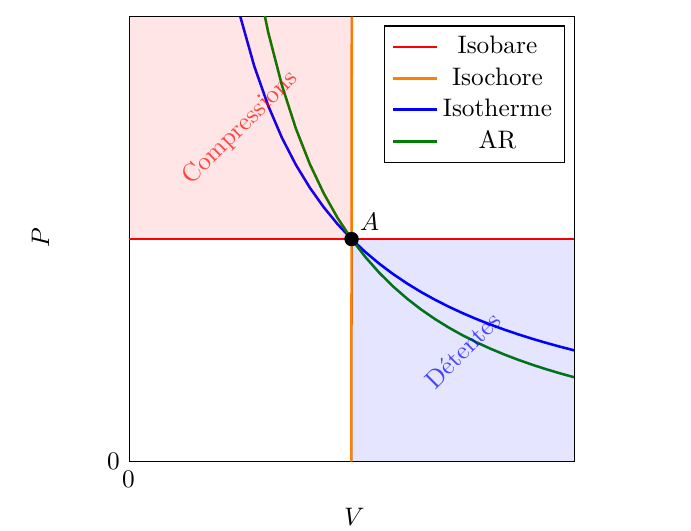
\includegraphics[width = \textwidth]{schema1.png}
		\end{proposition}
	\end{minipage}
	
	
\end{document}